% Results -- handbook section 2.3 requires this coverage
% Primary and secondary metrics, cost, and the qualitative evidence.

\section{Results}

%----------------------------------------------------------
\begin{frame}{Main Comparison}
\begin{table}
\centering
\caption{Main comparison.}
\label{tab:results}
\scriptsize
\begin{tabular}{lrrrrrcc}
\toprule
\textbf{Configuration} & \textbf{Params} & \textbf{s/ep} & \textbf{h} & \textbf{ms@1} & \textbf{GB} & \textbf{Val mIoU} & \textbf{Test mIoU} \\
\midrule
DeepLabV3-ResNet50      & 39{,}638{,}355 & 739.9 & 8.22 & 72.3 & 4.37 & \textit{0.6665} & \textit{0.7076} \\
\textbf{DeepLabV3-MobileNetV3} & 11{,}024{,}963 & 140.4 & 1.52 & 15.2 & 3.41 & $\mathbf{0.6136 \pm 0.0051}$ & $\mathbf{0.6180 \pm 0.0049}$ \\
\quad frozen backbone   &  8{,}053{,}011 &  95.3 & 0.84 & 14.7 & 3.41 & $0.4961 \pm 0.0049$ & $0.5003 \pm 0.0088$ \\
\quad Dice loss         & 11{,}024{,}963 & 150.5 & 0.50 & 14.9 & 3.41 & $0.4958 \pm 0.0045$ & $0.4983 \pm 0.0123$ \\
U-Net, from scratch     &  7{,}763{,}635 & 260.2 & 2.89 & 22.6 & 6.57 & $0.4836 \pm 0.0154$ & $0.4702 \pm 0.0071$ \\
\bottomrule
\end{tabular}
\end{table}

\vspace{-0.15cm}
\footnotesize
\begin{itemize}
    \item \textbf{One large effect, three ways of losing it.} Only the fully fine-tuned pretrained
          model separates. The other three three-seed arms are \textbf{mutually
          indistinguishable}, within 0.0126 of each other; the frozen and Dice arms differ by
          \textbf{0.0003}.
    \item \textbf{Pixel accuracy ranks them the other way round:} U-Net 0.9202 beats frozen 0.8959
          and Dice 0.8982, while losing on mIoU. Exactly what the EDA predicted.
\end{itemize}
\end{frame}

%----------------------------------------------------------
\begin{frame}{Decision Rule Applied}
\small
\begin{table}
\centering
\caption{Every pairwise comparison, on validation mIoU.}
\begin{tabular}{llc}
\toprule
\textbf{Comparison} & \textbf{Verdict} & \textbf{Margin} \\
\midrule
DeepLabV3 vs.\ U-Net           & DeepLabV3 better        & 0.1301 \\
DeepLabV3 vs.\ frozen backbone & Full fine-tuning better & 0.1175 \\
DeepLabV3 vs.\ Dice loss       & Cross-entropy better    & 0.1178 \\
\midrule
U-Net vs.\ frozen backbone     & \textbf{Indistinguishable} & 0.0126 \\
U-Net vs.\ Dice loss           & \textbf{Indistinguishable} & 0.0123 \\
Frozen vs.\ Dice loss          & \textbf{Indistinguishable} & 0.0003 \\
\midrule
Anything vs.\ ResNet50         & Indicative only, one seed & n/a \\
\bottomrule
\end{tabular}
\end{table}

\begin{block}{Why three seeds were necessary}
The U-Net's seed spread is $0.0154$, \textbf{three times} that of the pretrained arms, with seeds
at $0.4687$, $0.4824$, $0.4995$. Its \emph{best} seed would have tied the frozen arm; its worst
would have lost clearly. A one-seed study could have reported either outcome.
\end{block}
\end{frame}

%----------------------------------------------------------
\begin{frame}{Training Behaviour}
\begin{figure}
\centering
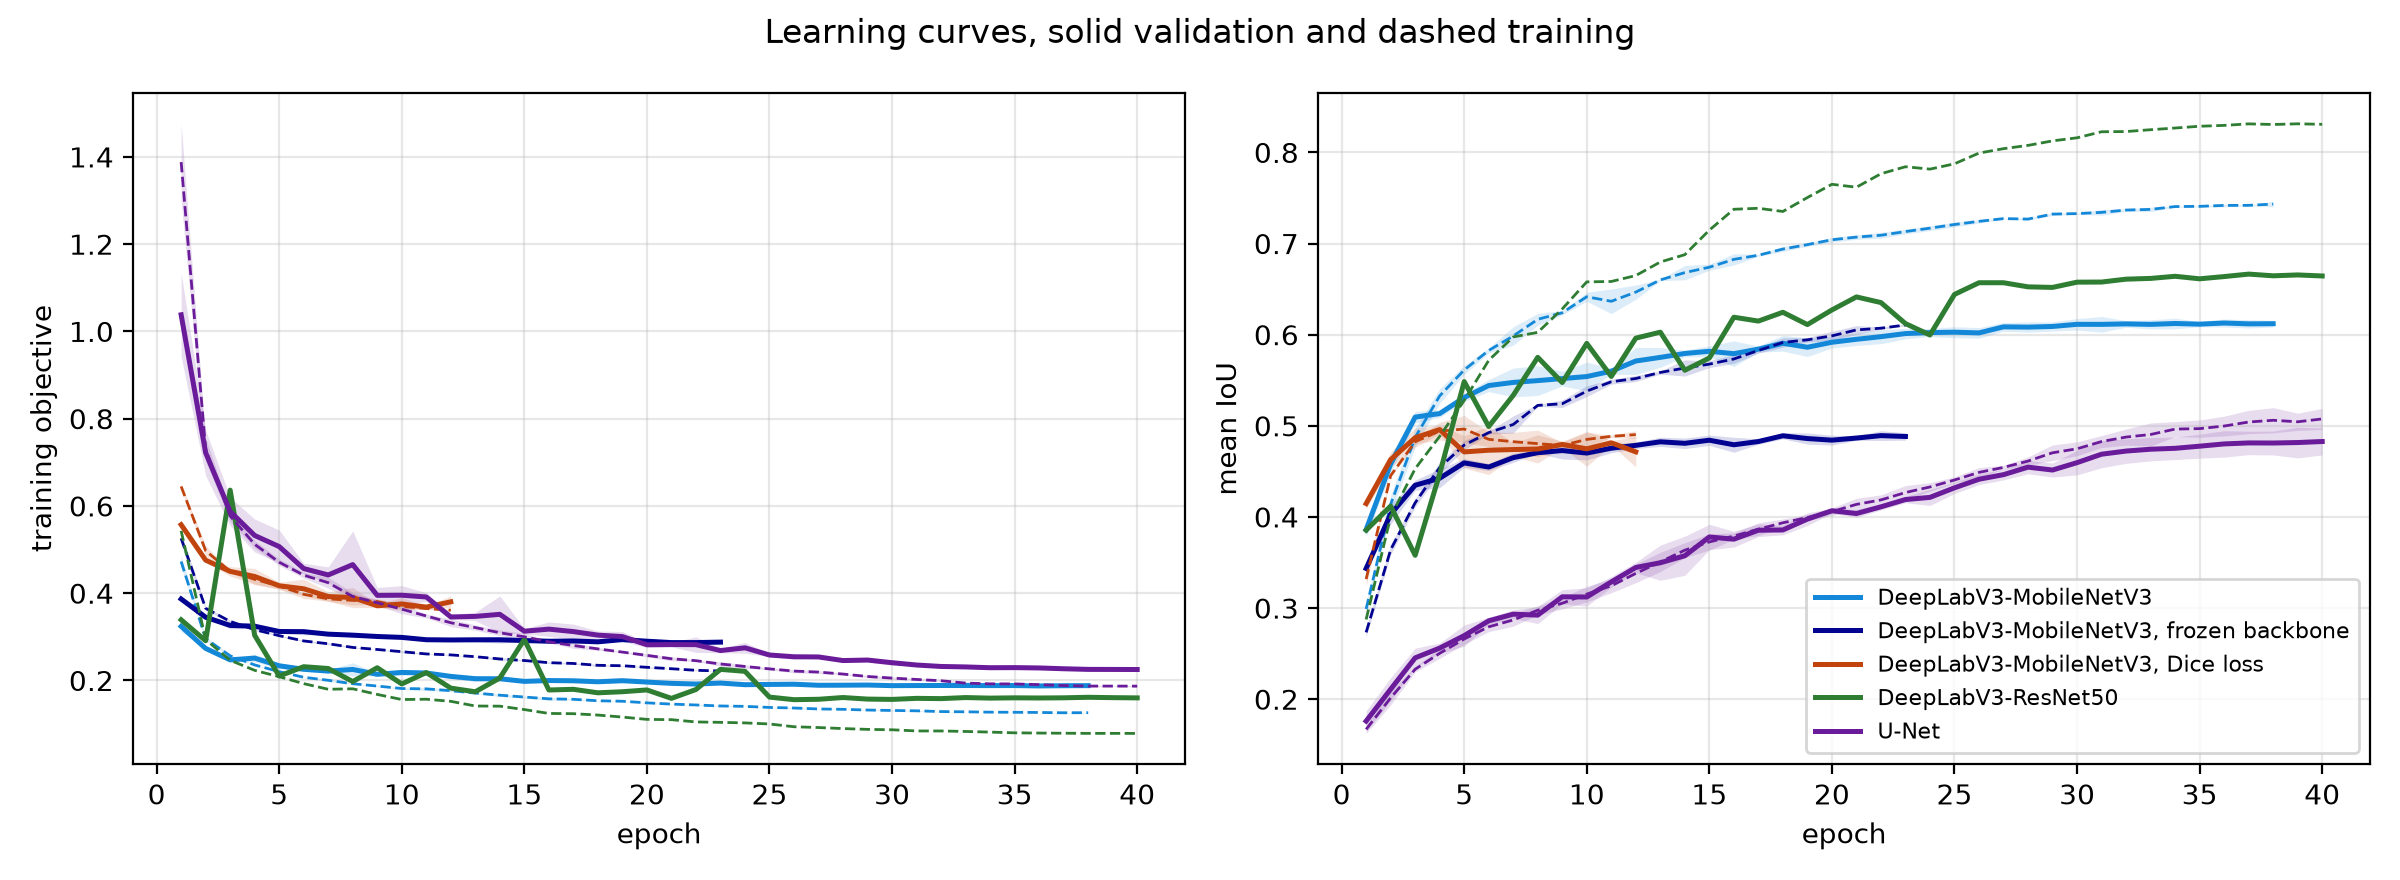
\includegraphics[width=0.80\textwidth]{../results/figures/all/learning_curves.png}
\caption{Solid validation, dashed training; the left axis mixes two objectives.}
\label{fig:curves}
\end{figure}

\vspace{-0.3cm}
\footnotesize
\begin{itemize}
    \item \textbf{Budget was right for DeepLabV3:} best epoch 30/31/35 of 38/39/40, flat from
          about epoch 32.
    \item \textbf{The U-Net is undertrained:} best epoch 38/40/39 of 40, still rising at the last
          epoch. \textbf{0.4836 is a floor}, so the margin over it is an upper bound.
    \item \textbf{Dice peaked at epoch 4} on all three seeds and stopped at 12.
\end{itemize}
\end{frame}

%----------------------------------------------------------
\begin{frame}{Where the Difference Appears}
\vspace{-0.2cm}
\begin{figure}
\centering
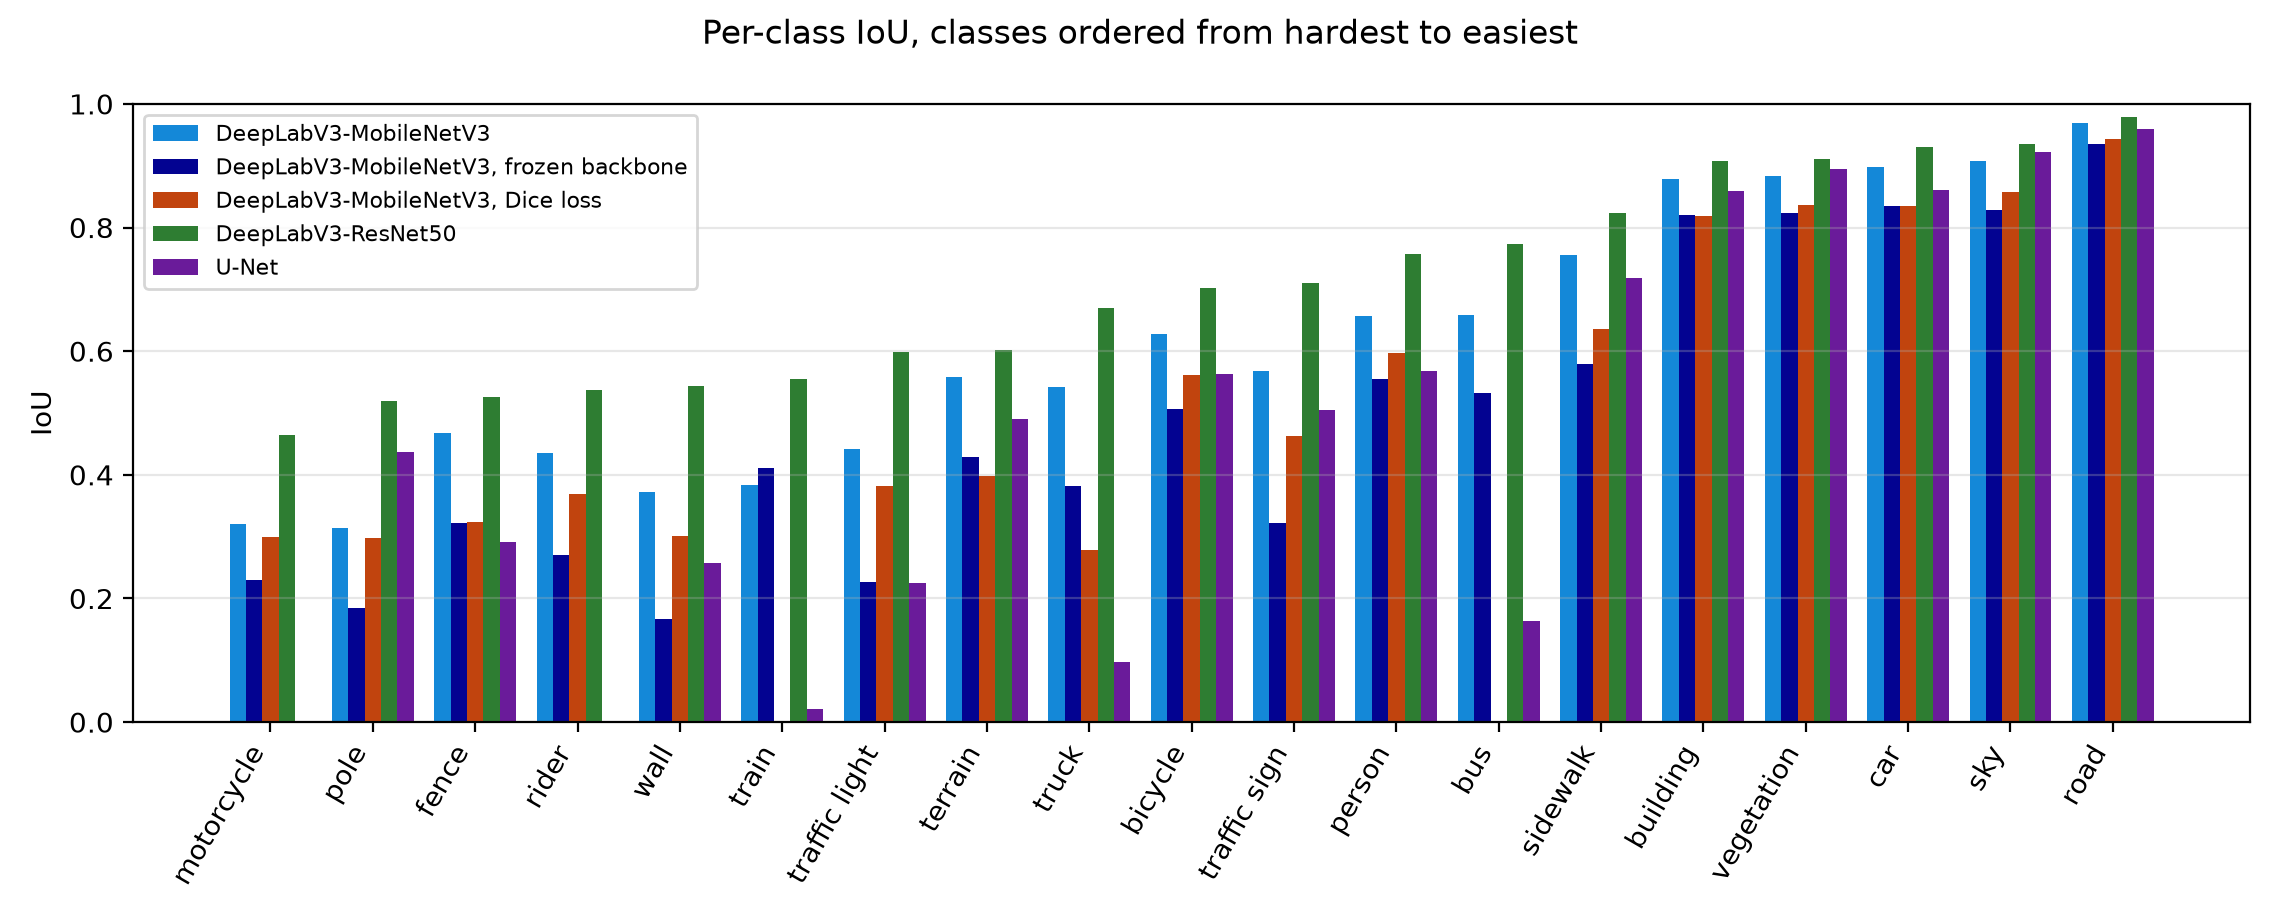
\includegraphics[width=0.80\textwidth]{../results/figures/all/per_class_iou_test.png}
\caption{Per-class IoU on test, hardest class first.}
\label{fig:per-class}
\end{figure}

\vspace{-0.3cm}
\footnotesize
\begin{itemize}
    \item \textbf{Frozen loses on all 19 classes}, but very unevenly: 0.027 on road, 0.044 on car
          against 0.215 on truck, 0.213 on traffic sign and 0.173 on traffic light.
          A frozen backbone keeps what fills a street scene and loses what does not.
    \item \textbf{Pretraining is not uniformly better.} The from-scratch U-Net \emph{beats}
          DeepLabV3, with separated intervals, on \textbf{pole} (0.4126 vs.\ 0.3277), sky and
          vegetation.
\end{itemize}
\end{frame}

%----------------------------------------------------------
\begin{frame}{Compute Cost}
\small
\begin{columns}[T]
\begin{column}{0.52\textwidth}
\begin{block}{The U-Net is Pareto-dominated}
30\% \emph{fewer} parameters than DeepLabV3, yet
\begin{itemize}
    \item $1.9\times$ the seconds per epoch,
    \item $1.5\times$ the latency at batch 1, $2.7\times$ at batch 8,
    \item $1.9\times$ the peak memory (6.57 vs.\ 3.41 GB),
    \item and $0.130$ lower mIoU.
\end{itemize}
Parameter count is \textbf{not} a proxy for cost: its convolutions run at full resolution and its
decoder holds every encoder map alive.
\end{block}
\end{column}
\begin{column}{0.46\textwidth}
\begin{block}{Freezing is a training-only saving}
$0.84$\,h against $1.52$\,h, a 45\% saving, for $0.118$ mIoU.

Smaller than it sounds: \textbf{73\% of parameters stay trainable}, because the ASPP head holds
8.05M against the backbone's 2.97M.

\textbf{Inference cost is identical} (14.7 vs.\ 15.2 ms), because the same forward pass runs either way.
\end{block}
\begin{alertblock}{Scaling the backbone}
ResNet50: $+0.0529$ val mIoU for $5.3\times$ s/epoch and $4.8\times$ latency. One ResNet50 run
costs more than the nine MobileNetV3 runs combined.
\end{alertblock}
\end{column}
\end{columns}
\end{frame}

%----------------------------------------------------------
\begin{frame}{Qualitative Results}
\vspace{-0.2cm}
\begin{figure}
\centering
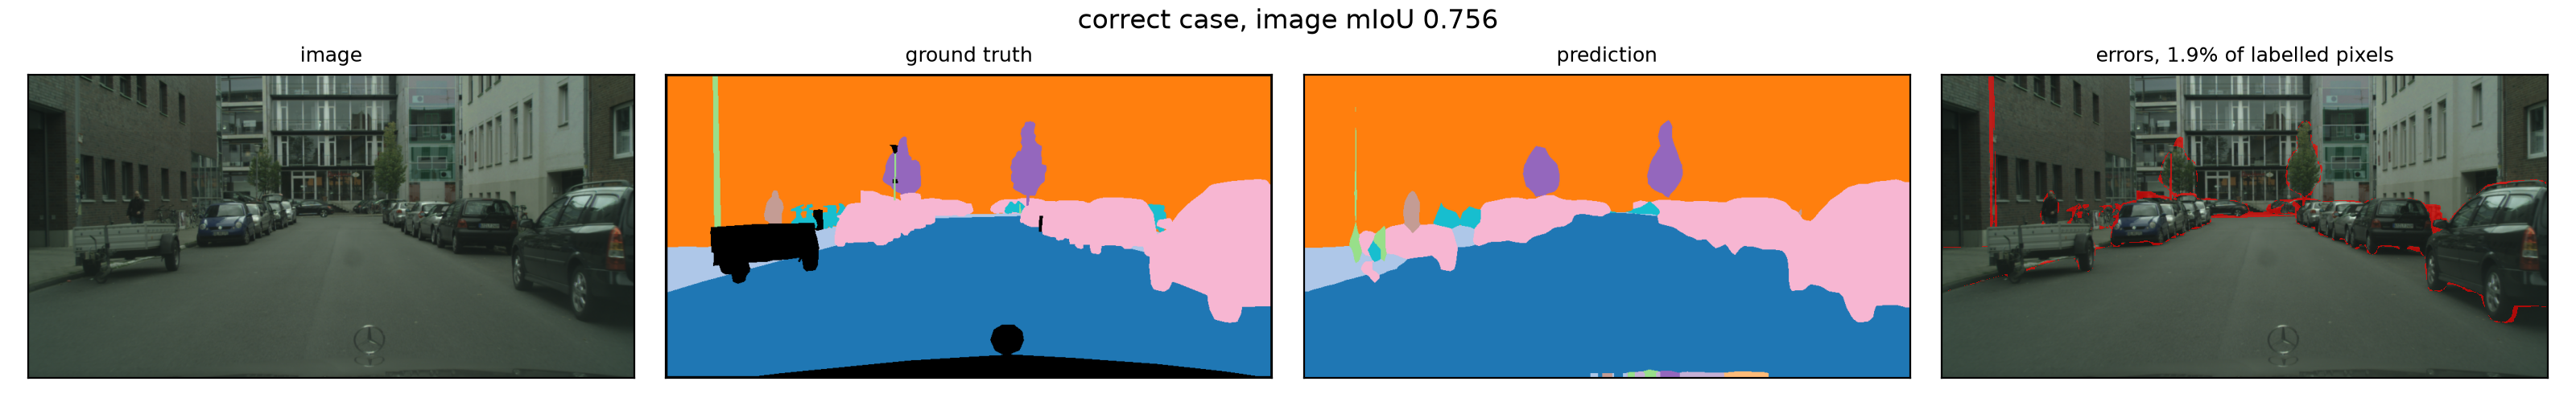
\includegraphics[width=0.92\textwidth]{images/example_correct.png}

\vspace{1mm}
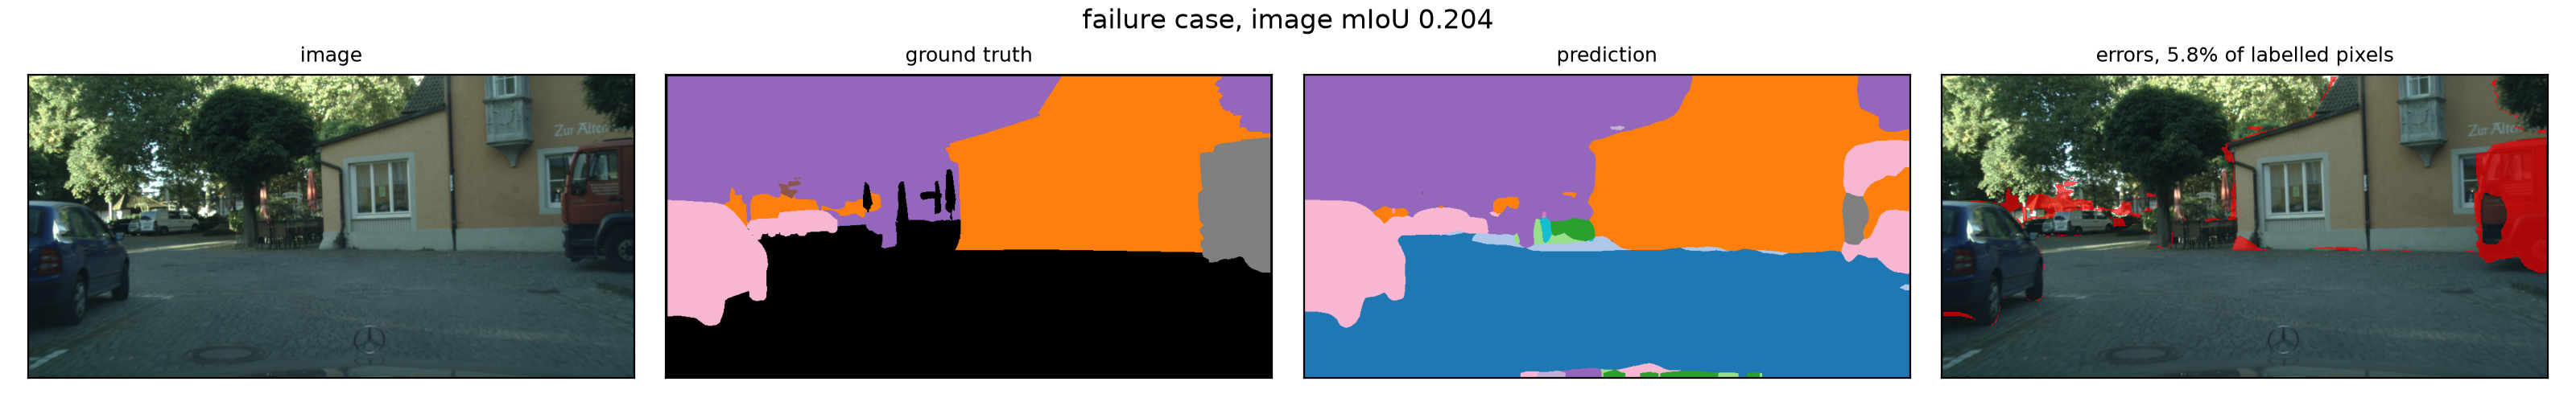
\includegraphics[width=0.92\textwidth]{images/example_failure.png}
\caption{Best image (0.756 mIoU) above, worst (0.204) below.}
\label{fig:examples}
\end{figure}

\vspace{-0.3cm}
\footnotesize
\begin{itemize}
    \item \textbf{Correct case:} the error is a thin outline tracing every boundary, so the model
          knows \emph{what}, and is imprecise about \emph{where}.
    \item \textbf{The failure case has only 5.8\% of labelled pixels wrong}, \emph{below} the
          6.7\% split average, yet is the worst image in the split. Most of the courtyard carries
          the ignore label, so few pixels are scored and each class has tiny support.
          \textbf{Per-image mIoU and per-image error are only loosely coupled.}
\end{itemize}
\end{frame}
